\documentclass{article}
\usepackage{graphicx} % Required for inserting images
\usepackage{amsmath}
\usepackage{hyperref}
\usepackage[margin=1cm]{geometry}
\usepackage{tikz}
\usetikzlibrary{shapes, arrows, positioning}


\title{StarkPredict: A Blockchain-Enabled Predictive Maintenance Platform Using StarkNet for Industrial IoT Data Security}
\author{Francisco J. Solis-Munoz}
\date{June 2024}

\begin{document}

\maketitle

Predictive maintenance is vital for industrial operations to minimize downtime and enhance equipment performance. This paper introduces \textit{StarkPredict}, a predictive maintenance platform utilizing StarkNet's blockchain technology to secure and manage Industrial Internet of Things (IIoT) data. \textit{StarkPredict} integrates real-time monitoring, advanced predictive analytics, and automated maintenance workflows via smart contracts, ensuring reliable and tamper-proof data.

The system features a Node.js backend, MongoDB storage, a React.js frontend, and StarkNet integration for decentralized data management. Machine learning models analyze historical and real-time sensor data to predict equipment failures and recommend maintenance actions. The web interface provides dashboards, user management, and mobile access, offering a user-friendly experience for industrial managers.

Our implementation shows significant improvements in predictive maintenance accuracy, data security, and operational efficiency compared to traditional methods. \textit{StarkPredict} addresses IIoT data security challenges and sets the stage for future industrial maintenance innovations. This paper details the system architecture, deployment, performance, and impact, highlighting \textit{StarkPredict}'s potential to revolutionize industrial predictive maintenance through blockchain technology. The findings suggest substantial benefits in operational reliability and cost reduction, establishing \textit{StarkPredict} as a pioneering platform in the IIoT landscape.

\textbf{Keywords:} Predictive Maintenance, Blockchain, StarkNet, Industrial IoT (IIoT), Data Security, Smart Contracts
\section{Introduction}
In the modern industrial landscape, predictive maintenance has emerged as a critical strategy for minimizing equipment downtime and optimizing performance. Traditional maintenance approaches, which are often reactive, lead to unplanned downtimes, increased operational costs, and potential safety hazards. Predictive maintenance, on the other hand, leverages data from Industrial Internet of Things (IIoT) devices to forecast equipment failures before they occur, allowing for timely and efficient maintenance actions \cite{lee2018predictive, kang2016smart}.

However, the implementation of predictive maintenance in industrial settings faces significant challenges, particularly in terms of data security and integrity. IIoT systems generate vast amounts of sensitive data, which must be securely collected, stored, and analyzed to ensure accurate predictions. The traditional centralized data management systems are prone to security breaches and data tampering, which can compromise the reliability of the maintenance predictions \cite{atzori2010internet}.

Blockchain technology offers a promising solution to these challenges by providing a decentralized, immutable ledger that ensures data integrity and security. StarkNet, a Layer 2 scaling solution on Ethereum, enhances these benefits with its high throughput, low costs, and native support for account abstraction \cite{ben2019starknet}. By integrating blockchain with IIoT, it is possible to create a robust and secure platform for predictive maintenance.

This paper introduces \textit{StarkPredict}, a blockchain-enabled predictive maintenance platform that leverages StarkNet for secure and scalable data management. The platform integrates real-time monitoring, advanced predictive analytics, and automated maintenance workflows through smart contracts. \textit{StarkPredict} addresses the current challenges in IIoT data security, ensuring that the data used for maintenance predictions is reliable and tamper-proof.

The rest of this paper is organized as follows: Section 2 reviews related work in the field of predictive maintenance and blockchain applications in IIoT. Section 3 describes the system architecture of \textit{StarkPredict}, including its backend, frontend, and blockchain integration. Section 4 details the predictive maintenance model and its implementation. Section 5 discusses the web interface and user experience. Section 6 covers the implementation and deployment process. Section 7 presents the results and performance analysis, and Section 8 concludes the paper with a discussion on the impact and future work.

\section{Related Work}

The integration of blockchain technology with Industrial Internet of Things (IIoT) systems for predictive maintenance is an emerging field that addresses challenges in data security, integrity, and operational efficiency. This section reviews the current state of research and development in this area, highlighting relevant studies and identifying gaps that the \textit{StarkPredict} platform aims to address.
Predictive Maintenance in IIoT

\noindent\textbf{Predictive Maintenance in IIoT}

Predictive maintenance utilizes IIoT data to anticipate equipment failures, allowing for proactive maintenance actions that reduce downtime and operational costs. Various studies have explored the application of machine learning and data analytics in predictive maintenance. Lee et al. \cite{lee2018predictive} demonstrated the use of machine learning models to predict equipment failures in manufacturing systems, highlighting significant improvements in maintenance scheduling and equipment reliability. Similarly, Kang et al. \cite{kang2016smart} reviewed smart manufacturing technologies, emphasizing the role of predictive maintenance in enhancing operational efficiency.

Rao et al. \cite{rao2016predictive} explored data-driven predictive maintenance strategies in the context of smart manufacturing, demonstrating how data analytics can improve decision-making processes. Jardine et al. \cite{jardine2006review} provided a comprehensive review of prognostics and health management in predictive maintenance, underscoring the importance of accurate failure prediction models.
Blockchain for Data Security in IIoT

\noindent\textbf{Blockchain for Data Security in IIoT}

Blockchain technology offers a decentralized and secure method for managing IIoT data, addressing issues related to data integrity and tampering. Atzori et al. \cite{atzori2010internet} discussed the potential of blockchain to enhance the security of IoT systems by providing a tamper-proof ledger for data transactions. The immutability and transparency of blockchain make it an ideal solution for securing IIoT data, as it ensures that data remains unaltered and traceable.

Dorri et al. \cite{dorri2017blockchain} proposed a lightweight blockchain framework for securing IoT data, demonstrating its effectiveness in enhancing data privacy and security. Christidis and Devetsikiotis \cite{christidis2016blockchains} reviewed blockchain applications in IoT, highlighting the potential of blockchain to provide secure and decentralized data management solutions.
Integration of Blockchain with IIoT

\noindent\textbf{Integration of Blockchain with IIoT}

Several studies have explored the integration of blockchain with IIoT to enhance data security and enable new applications. Ben-Sasson et al. \cite{ben2019starknet} introduced StarkNet, a Layer 2 scaling solution on Ethereum, which offers high throughput and low costs while maintaining the security benefits of blockchain. This integration allows for the creation of decentralized applications that can securely manage and analyze IIoT data.

Zheng et al. \cite{zheng2017overview} provided an overview of blockchain technology and its applications, including its use in IoT and industrial contexts. Xu et al. \cite{xu2019blendcac} developed BlendCAC, a blockchain-based access control framework for IoT, which enhances data security and access management.
Existing Solutions and Gaps

\noindent\textbf{Existing Solutions and Gaps}

Existing solutions for predictive maintenance and IIoT data security often rely on centralized systems, which are vulnerable to security breaches and data tampering. Blockchain-based approaches, such as those discussed by IBM and other researchers \cite{ibm2019blockchain}, provide a more secure and decentralized alternative. However, there is a need for scalable and efficient platforms that can seamlessly integrate blockchain with IIoT systems, providing real-time monitoring and predictive analytics.

Lin and Wen \cite{lin2018blockchain} explored blockchain-based frameworks for IoT applications, highlighting challenges in scalability and interoperability. Novo \cite{novo2018blockchain} proposed a blockchain-based framework for IoT that addresses security and scalability issues, but emphasized the need for further research in integrating blockchain with IIoT.

The \textit{StarkPredict} platform aims to address these gaps by leveraging StarkNet's blockchain technology to ensure data integrity and security while providing advanced predictive maintenance capabilities. By integrating machine learning models and smart contracts, \textit{StarkPredict} offers a robust solution for industrial predictive maintenance.

\section{System Architecture}

The system architecture of the \textit{StarkPredict} platform integrates several components to provide a robust and secure predictive maintenance solution. The architecture consists of a backend for data processing, a frontend for user interaction, and a blockchain layer for data security and integrity. The integration of these components ensures real-time monitoring, predictive analytics, and automated maintenance workflows. A diagram of the system architecture is observed in \autoref{fig:system_architecture}.

\subsection{Overall Architecture}

The \textit{StarkPredict} architecture can be divided into the following main components:

\begin{enumerate}
    \item IIoT Devices: Sensors and devices deployed in the industrial environment to collect data.
    \item Data Processing Backend: Node.js server for handling API requests, data processing, and interfacing with the blockchain.
    \item Database: MongoDB for storing IIoT data and user information.
    \item Blockchain Layer: StarkNet for decentralized data storage and smart contract execution.
    \item Machine Learning Models: Algorithms for predictive analytics.
    \item Web Interface: React.js frontend for user interaction and data visualization.
\end{enumerate}

\begin{figure}
    \centering
    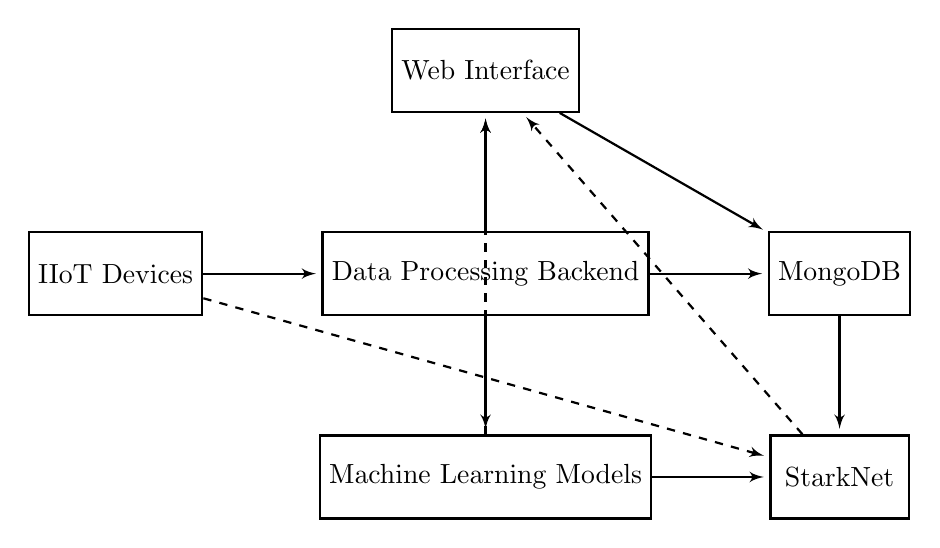
\begin{tikzpicture}[
    node distance=1.5cm, auto,
    block/.style ={rectangle, draw=black, thick, fill=white, text centered, minimum height=3em, minimum width=5em},
    line/.style ={draw, thick, -latex', shorten >=2pt},
]

% Nodes
\node [block] (iot) {IIoT Devices};
\node [block, right=of iot] (backend) {Data Processing Backend};
\node [block, right=of backend] (database) {MongoDB};
\node [block, below=of backend] (ml) {Machine Learning Models};
\node [block, below=of database] (blockchain) {StarkNet};
\node [block, above=of backend] (frontend) {Web Interface};

% Lines
\path [line] (iot) -- (backend);
\path [line] (backend) -- (database);
\path [line] (backend) -- (ml);
\path [line] (ml) -- (blockchain);
\path [line] (database) -- (blockchain);
\path [line] (backend) -- (frontend);
\path [line] (frontend) -- (database);

% Additional lines to show interactions
\path [line, dashed] (iot) -- (blockchain);
\path [line, dashed] (ml) -- (frontend);
\path [line, dashed] (blockchain) -- (frontend);

\end{tikzpicture}


    \caption{Overall System Architecture of \textit{StarkPredict}}
    \label{fig:system_architecture}
\end{figure}

\subsection{IIoT Devices}

IIoT devices are deployed throughout the industrial environment to collect data on various parameters such as temperature, vibration, noise, and operational status. These devices continuously transmit data to the data processing backend.

\subsection{Data Processing Backend}

The backend, built using Node.js, handles API requests, processes the incoming data from IIoT devices, and interfaces with the blockchain layer. It ensures the efficient processing of large volumes of data and prepares it for storage and analysis.

\subsection{Database}

MongoDB is used to store IIoT data and user information. It provides a scalable and flexible data storage solution that can handle the high throughput requirements of the system. Example of data that should be stored would be raw sensor data, aggregated data, and maintenance logs.

\subsection{Blockchain Layer}

StarkNet is used for decentralized data storage and smart contract execution. It ensures data integrity and security by providing an immutable and transparent ledger. Smart contracts automate maintenance workflows and ensure that data transactions are secure and tamper-proof. Example of data that would be stored would be critical maintenance records and audit logs.

\subsection{Machine Learning Models}

Machine learning models analyze the historical and real-time data collected from IIoT devices to predict equipment failures and recommend maintenance actions. These models are integrated into the backend to provide real-time predictive analytics.

\subsection{Web Interface}

The web interface, built using React.js, provides users with an interactive dashboard to monitor equipment status, view predictive analytics, and manage maintenance schedules. It ensures a user-friendly experience for industrial managers and maintenance teams.


\bibliographystyle{IEEEtran}
\bibliography{references}
\end{document}

